\chapter{Code Coverage}
\begin{tiny}
	SS
\end{tiny}


Um den Code Coverage unseres Systems \textbf{OfCourse} zu testen, benutzten wir das Java Plugin ECLEmma und führten alle Tests mithilfe einer JUnit TestSuit auf einmal aus.
Es ist uns leider nicht gelungen, dass ECLEmma auf den Code zugreifen kann. Dadurch, dass unsere JUnit Tests mit einem WebDriver laufen erkannt er nicht welche Methoden im Hintergrund ausgeführt worden sind. 
Dies sieht man sehr deutlich an dem Ergebnis.

\centering
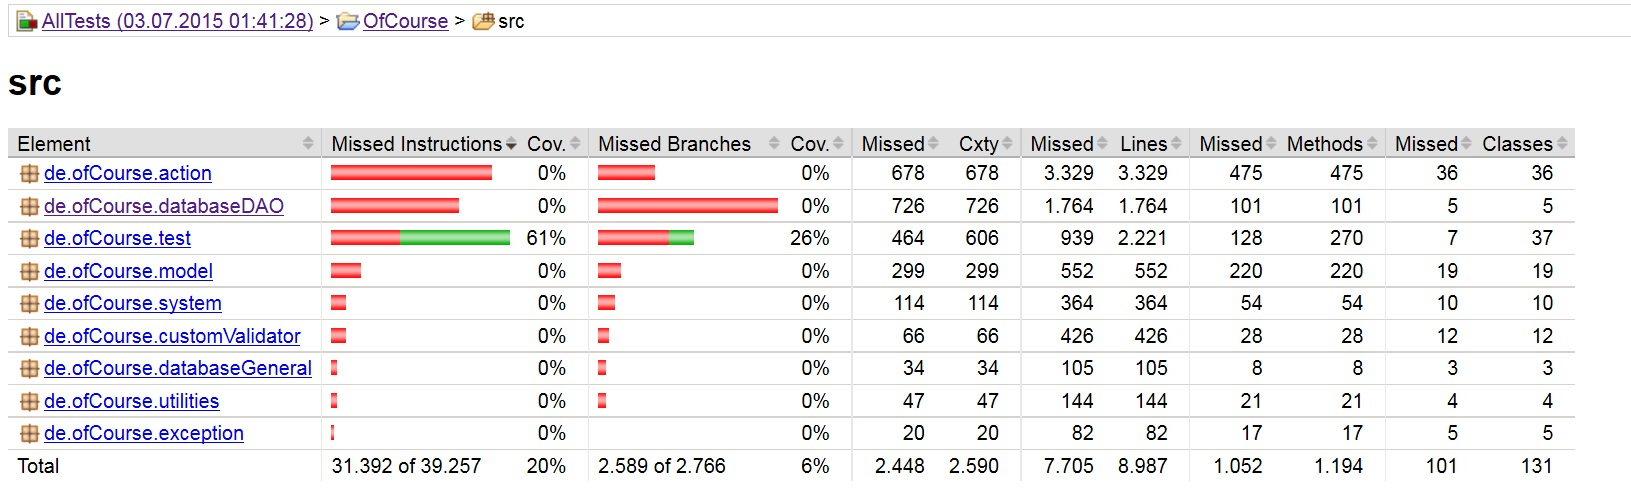
\includegraphics[width=1\linewidth]{img/CodeCoverage}
\caption{CodeCoverage}
\label{fig:CodeCoverage}